\subsection{Strategy}
\subsubsection{Định nghĩa}
Strategy (Chiến lược) là một mẫu thiết kế hành vi cho phép đối tượng thay đổi thuật toán được sử dụng trong quá trình thực thi một hành động cụ thể mà không ảnh hưởng đến các đối tượng khác hoặc cấu trúc của chúng. Mẫu này tách rời thuật toán khỏi đối tượng sử dụng nó, giúp tăng tính linh hoạt và tái sử dụng trong việc áp dụng các thuật toán khác nhau.
\subsubsection{Cách sử dụng}
Ta có thể sử dụng Strategy Pattern trong các trường hợp sau:
\begin{itemize}
    \item Khi có một hành động cần thực hiện, nhưng có nhiều thuật toán khác nhau có thể được áp dụng, và cần linh hoạt trong việc chọn thuật toán tại thời điểm chạy.
    \item Khi muốn tránh sự phức tạp của việc sử dụng nhiều câu lệnh điều kiện (if-else hoặc switch-case) để chọn thuật toán.
    \item Khi muốn tránh sự phức tạp của việc sử dụng nhiều câu lệnh điều kiện (if-else hoặc switch-case) để chọn thuật toán.
\end{itemize}
\subsubsection{Cấu trúc}
\begin{center}
    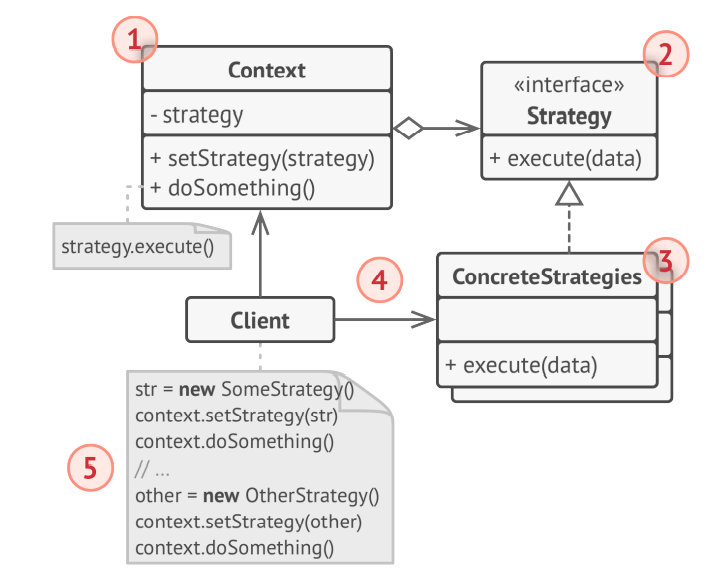
\includegraphics[scale=0.6]{image/behavioral/strategy.png}
\end{center}
\subsubsection{Ưu điểm và Nhược điểm}
Ta có rất nhiều ưu nhược điểm như sau:\\\\
Ưu điểm:
\begin{itemize}
    \item Linh hoạt và dễ dàng thay đổi thuật toán tại thời điểm chạy.
    \item Khi thay đổi thuật toán hoặc khi thêm mới thuật toán, không cần thay đổi code phần context.
    \item Có thể thay thế việc kế thừa bằng việc encapsulate thuật toán.
\end{itemize}
Nhược điểm:
\begin{itemize}
    \item Tăng số lượng các lớp và đối tượng, đặc biệt khi có nhiều thuật toán khác nhau.
    \item Cần phải hiểu rõ các thuật toán khác nhau để chọn và sử dụng một cách phù hợp.
\end{itemize}
\subsubsection{Code Example}
\begin{itemize}
    \item Có một interface và 2 concrete class thực hiện hóa 2 hàm sort.
    \item Một class Sorter có Strategy sort trong đó.
\end{itemize}
\begin{lstlisting}
#include <iostream>

// Strategy interface
class SortingStrategy {
public:
    virtual void sort(int* arr, int size) = 0;
};

// Concrete strategies
class QuickSortStrategy : public SortingStrategy {
public:
    void sort(int* arr, int size) override {
        std::cout << "Sorting using Quick Sort." << std::endl;
        // Perform Quick Sort algorithm
    }
};

class MergeSortStrategy : public SortingStrategy {
public:
    void sort(int* arr, int size) override {
        std::cout << "Sorting using Merge Sort." << std::endl;
        // Perform Merge Sort algorithm
    }
};

// Context class
class Sorter {
private:
    SortingStrategy* strategy;

public:
    void setStrategy(SortingStrategy* sortingStrategy) {
        strategy = sortingStrategy;
    }

    void sortArray(int* arr, int size) {
        strategy->sort(arr, size);
    }
};

int main() {
    int arr[] = {5, 2, 8, 1, 9};
    int size = sizeof(arr) / sizeof(arr[0]);

    Sorter sorter;

    QuickSortStrategy quickSortStrategy;
    MergeSortStrategy mergeSortStrategy;

    sorter.setStrategy(&quickSortStrategy);
    sorter.sortArray(arr, size);

    sorter.setStrategy(&mergeSortStrategy);
    sorter.sortArray(arr, size);

    return 0;
}

\end{lstlisting}
Ở hàm main, ta tạo ra 2 kiểu sort rồi thực hiện tuần tự 2 loại sort.\\
\newline
\textbf{Kết quả:}
\begin{lstlisting}
Sorting using Quick Sort.
Sorting using Merge Sort.
\end{lstlisting}
\subsubsection{Các Pattern liên quan}
\begin{itemize}
    \item Bridge có cấu trúc gống Strategy dựa trên composition.
    \item Command: giống nhau ở chỗ tham số hóa một đối tượng và hành động.
    \item State: là một bản mở rộng của Strategy.
\end{itemize}